%% AMS-LaTeX Created with the Wolfram Language : www.wolfram.com

\documentclass{article}
\usepackage{amsmath, amssymb, graphics, setspace}

\newcommand{\mathsym}[1]{{}}
\newcommand{\unicode}[1]{{}}

\newcounter{mathematicapage}
\begin{document}

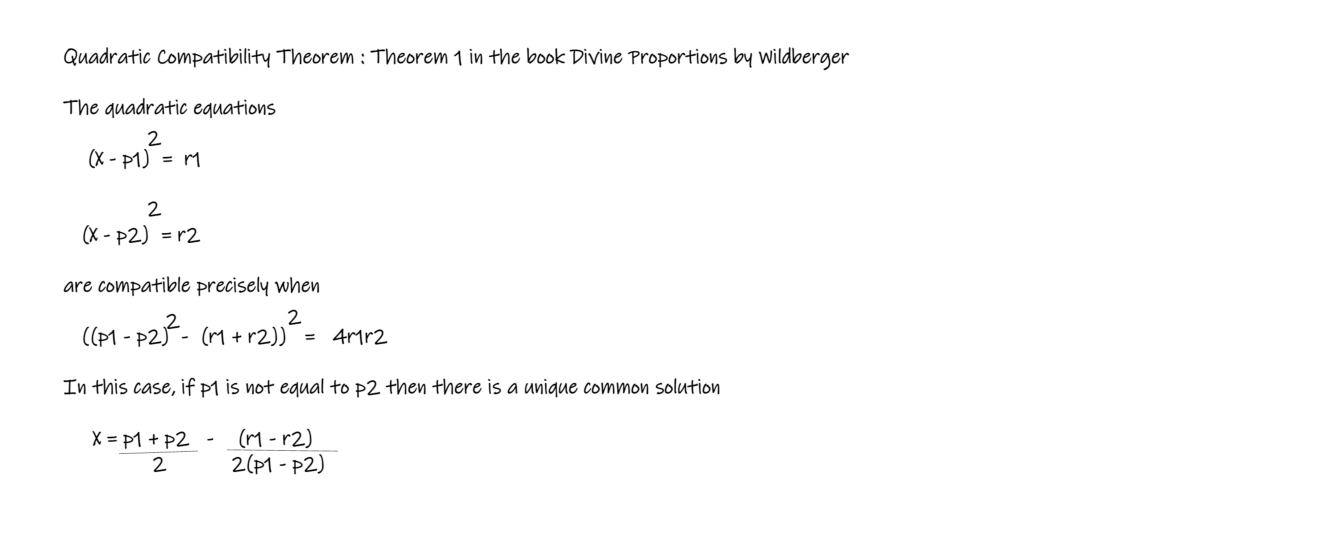
\includegraphics{quadreaOfHyperbolicProjectiveQuadranglelProofPart_1_gr1.eps}

Create a Mathematica function for unique common solution of a pair of compatible quadratic equations.

\begin{doublespace}
\noindent\(\pmb{X[\text{p1$\_$},\text{r1$\_$},\text{p2$\_$},\text{r2$\_$}]\text{:=}((\text{p1}+\text{p2})/2)-(\text{r1}-\text{r2})/(2(\text{p1}-\text{p2}))}\)
\end{doublespace}

Substitute values for p1, r1, p2 and r2 from quadratic equations (1) and (2) above to compute the qadrea B .

\begin{doublespace}
\noindent\(\pmb{B=X\left[q_{12}q_{23}S_2+q_{34}q_{41}S_4,4q_{12}q_{23}q_{34}q_{41}\left(1-S_1\right)\left(1-S_3\right),q_{12}q_{41}S_1+q_{23}q_{34}S_3,4q_{12}q_{23}q_{34}q_{41}\left(1-S_2\right)\left(1-S_4\right)\right]}\)
\end{doublespace}

\begin{doublespace}
\noindent\(-\frac{4 q_{12} q_{23} q_{34} q_{41} \left(1-S_1\right) \left(1-S_3\right)-4 q_{12} q_{23} q_{34} q_{41} \left(1-S_2\right) \left(1-S_4\right)}{2
\left(-q_{12} q_{41} S_1+q_{12} q_{23} S_2-q_{23} q_{34} S_3+q_{34} q_{41} S_4\right)}+\frac{1}{2} \left(q_{12} q_{41} S_1+q_{12} q_{23} S_2+q_{23}
q_{34} S_3+q_{34} q_{41} S_4\right)\)
\end{doublespace}



The proof employs the quadratic compatibility theorem. We will show that equations (1) and (2) above are compatible since they meet the criteria
for being compatible from the quadratic compatibility theorem. 

Perform compatibility check:

\begin{doublespace}
\noindent\(\pmb{\text{CompatibilityCheckLHS} [\text{p1$\_$},\text{r1$\_$},\text{p2$\_$},\text{r2$\_$}]\text{:=}\left((\text{p1}-\text{p2})^2-(\text{r1}+\text{r2})\right)^2}\)
\end{doublespace}

\begin{doublespace}
\noindent\(\pmb{\text{CompatibilityCheckRHS} [\text{p1$\_$},\text{r1$\_$},\text{p2$\_$},\text{r2$\_$}]\text{:=} 4*\text{r1}*\text{r2}}\)
\end{doublespace}

\begin{doublespace}
\noindent\(\pmb{\text{lhs} = \text{CompatibilityCheckLHS}\left[q_{12}q_{23}S_2+q_{34}q_{41}S_4,4q_{12}q_{23}q_{34}q_{41}\left(1-S_1\right)\left(1-S_3\right),q_{12}q_{41}S_1+q_{23}q_{34}S_3,\right.}\\
\pmb{\left.4q_{12}q_{23}q_{34}q_{41}\left(1-S_2\right)\left(1-S_4\right)\right]}\)
\end{doublespace}

\begin{doublespace}
\noindent\(\left(-4 q_{12} q_{23} q_{34} q_{41} \left(1-S_1\right) \left(1-S_3\right)-4 q_{12} q_{23} q_{34} q_{41} \left(1-S_2\right) \left(1-S_4\right)+\left(-q_{12}
q_{41} S_1+q_{12} q_{23} S_2-q_{23} q_{34} S_3+q_{34} q_{41} S_4\right){}^2\right){}^2\)
\end{doublespace}

\begin{doublespace}
\noindent\(\pmb{\text{rhs} = \text{CompatibilityCheckRHS}\left[q_{12}q_{23}S_2+q_{34}q_{41}S_4,4q_{12}q_{23}q_{34}q_{41}\left(1-S_1\right)\left(1-S_3\right),q_{12}q_{41}S_1+q_{23}q_{34}S_3,\right.}\\
\pmb{\left.4q_{12}q_{23}q_{34}q_{41}\left(1-S_2\right)\left(1-S_4\right)\right]}\)
\end{doublespace}

\begin{doublespace}
\noindent\(64 q_{12}^2 q_{23}^2 q_{34}^2 q_{41}^2 \left(1-S_1\right) \left(1-S_2\right) \left(1-S_3\right) \left(1-S_4\right)\)
\end{doublespace}

\begin{doublespace}
\noindent\(\pmb{\text{lhse} = \text{Expand}[\text{lhs}]}\)
\end{doublespace}

\begin{doublespace}
\noindent\(64 q_{12}^2 q_{23}^2 q_{34}^2 q_{41}^2-64 q_{12}^2 q_{23}^2 q_{34}^2 q_{41}^2 S_1+16 q_{12}^2 q_{23}^2 q_{34}^2 q_{41}^2 S_1^2-16 q_{12}^3
q_{23} q_{34} q_{41}^3 S_1^2+8 q_{12}^3 q_{23} q_{34} q_{41}^3 S_1^3+q_{12}^4 q_{41}^4 S_1^4-64 q_{12}^2 q_{23}^2 q_{34}^2 q_{41}^2 S_2+32 q_{12}^3
q_{23}^2 q_{34} q_{41}^2 S_1 S_2+32 q_{12}^2 q_{23}^2 q_{34}^2 q_{41}^2 S_1 S_2-16 q_{12}^3 q_{23}^2 q_{34} q_{41}^2 S_1^2 S_2+8 q_{12}^3 q_{23}
q_{34} q_{41}^3 S_1^2 S_2-4 q_{12}^4 q_{23} q_{41}^3 S_1^3 S_2-16 q_{12}^3 q_{23}^3 q_{34} q_{41} S_2^2+16 q_{12}^2 q_{23}^2 q_{34}^2 q_{41}^2 S_2^2+8
q_{12}^3 q_{23}^3 q_{34} q_{41} S_1 S_2^2-16 q_{12}^3 q_{23}^2 q_{34} q_{41}^2 S_1 S_2^2+6 q_{12}^4 q_{23}^2 q_{41}^2 S_1^2 S_2^2+8 q_{12}^3 q_{23}^3
q_{34} q_{41} S_2^3-4 q_{12}^4 q_{23}^3 q_{41} S_1 S_2^3+q_{12}^4 q_{23}^4 S_2^4-64 q_{12}^2 q_{23}^2 q_{34}^2 q_{41}^2 S_3+64 q_{12}^2 q_{23}^2
q_{34}^2 q_{41}^2 S_1 S_3-16 q_{12}^2 q_{23}^2 q_{34}^2 q_{41}^2 S_1^2 S_3+8 q_{12}^3 q_{23} q_{34} q_{41}^3 S_1^2 S_3-4 q_{12}^3 q_{23} q_{34} q_{41}^3
S_1^3 S_3+32 q_{12}^2 q_{23}^3 q_{34}^2 q_{41} S_2 S_3+32 q_{12}^2 q_{23}^2 q_{34}^2 q_{41}^2 S_2 S_3-16 q_{12}^2 q_{23}^3 q_{34}^2 q_{41} S_1 S_2
S_3-16 q_{12}^3 q_{23}^2 q_{34} q_{41}^2 S_1 S_2 S_3-16 q_{12}^2 q_{23}^2 q_{34}^2 q_{41}^2 S_1 S_2 S_3+4 q_{12}^3 q_{23}^2 q_{34} q_{41}^2 S_1^2
S_2 S_3+8 q_{12}^3 q_{23}^3 q_{34} q_{41} S_2^2 S_3-16 q_{12}^2 q_{23}^3 q_{34}^2 q_{41} S_2^2 S_3+4 q_{12}^3 q_{23}^3 q_{34} q_{41} S_1 S_2^2 S_3-4
q_{12}^3 q_{23}^4 q_{34} S_2^3 S_3-16 q_{12} q_{23}^3 q_{34}^3 q_{41} S_3^2+16 q_{12}^2 q_{23}^2 q_{34}^2 q_{41}^2 S_3^2+8 q_{12} q_{23}^3 q_{34}^3
q_{41} S_1 S_3^2-16 q_{12}^2 q_{23}^2 q_{34}^2 q_{41}^2 S_1 S_3^2+6 q_{12}^2 q_{23}^2 q_{34}^2 q_{41}^2 S_1^2 S_3^2-16 q_{12}^2 q_{23}^3 q_{34}^2
q_{41} S_2 S_3^2+8 q_{12} q_{23}^3 q_{34}^3 q_{41} S_2 S_3^2+4 q_{12}^2 q_{23}^3 q_{34}^2 q_{41} S_1 S_2 S_3^2+6 q_{12}^2 q_{23}^4 q_{34}^2 S_2^2
S_3^2+8 q_{12} q_{23}^3 q_{34}^3 q_{41} S_3^3-4 q_{12} q_{23}^3 q_{34}^3 q_{41} S_1 S_3^3-4 q_{12} q_{23}^4 q_{34}^3 S_2 S_3^3+q_{23}^4 q_{34}^4
S_3^4-64 q_{12}^2 q_{23}^2 q_{34}^2 q_{41}^2 S_4+32 q_{12}^2 q_{23}^2 q_{34}^2 q_{41}^2 S_1 S_4+32 q_{12}^2 q_{23} q_{34}^2 q_{41}^3 S_1 S_4+8 q_{12}^3
q_{23} q_{34} q_{41}^3 S_1^2 S_4-16 q_{12}^2 q_{23} q_{34}^2 q_{41}^3 S_1^2 S_4-4 q_{12}^3 q_{34} q_{41}^4 S_1^3 S_4+64 q_{12}^2 q_{23}^2 q_{34}^2
q_{41}^2 S_2 S_4-16 q_{12}^3 q_{23}^2 q_{34} q_{41}^2 S_1 S_2 S_4-16 q_{12}^2 q_{23}^2 q_{34}^2 q_{41}^2 S_1 S_2 S_4-16 q_{12}^2 q_{23} q_{34}^2
q_{41}^3 S_1 S_2 S_4+4 q_{12}^3 q_{23} q_{34} q_{41}^3 S_1^2 S_2 S_4+8 q_{12}^3 q_{23}^3 q_{34} q_{41} S_2^2 S_4-16 q_{12}^2 q_{23}^2 q_{34}^2 q_{41}^2
S_2^2 S_4+4 q_{12}^3 q_{23}^2 q_{34} q_{41}^2 S_1 S_2^2 S_4-4 q_{12}^3 q_{23}^3 q_{34} q_{41} S_2^3 S_4+32 q_{12}^2 q_{23}^2 q_{34}^2 q_{41}^2 S_3
S_4+32 q_{12} q_{23}^2 q_{34}^3 q_{41}^2 S_3 S_4-16 q_{12}^2 q_{23}^2 q_{34}^2 q_{41}^2 S_1 S_3 S_4-16 q_{12} q_{23}^2 q_{34}^3 q_{41}^2 S_1 S_3
S_4-16 q_{12}^2 q_{23} q_{34}^2 q_{41}^3 S_1 S_3 S_4+4 q_{12}^2 q_{23} q_{34}^2 q_{41}^3 S_1^2 S_3 S_4-16 q_{12}^2 q_{23}^3 q_{34}^2 q_{41} S_2 S_3
S_4-16 q_{12}^2 q_{23}^2 q_{34}^2 q_{41}^2 S_2 S_3 S_4-16 q_{12} q_{23}^2 q_{34}^3 q_{41}^2 S_2 S_3 S_4+24 q_{12}^2 q_{23}^2 q_{34}^2 q_{41}^2 S_1
S_2 S_3 S_4+4 q_{12}^2 q_{23}^3 q_{34}^2 q_{41} S_2^2 S_3 S_4+8 q_{12} q_{23}^3 q_{34}^3 q_{41} S_3^2 S_4-16 q_{12} q_{23}^2 q_{34}^3 q_{41}^2 S_3^2
S_4+4 q_{12} q_{23}^2 q_{34}^3 q_{41}^2 S_1 S_3^2 S_4+4 q_{12} q_{23}^3 q_{34}^3 q_{41} S_2 S_3^2 S_4-4 q_{23}^3 q_{34}^4 q_{41} S_3^3 S_4+16 q_{12}^2
q_{23}^2 q_{34}^2 q_{41}^2 S_4^2-16 q_{12} q_{23} q_{34}^3 q_{41}^3 S_4^2-16 q_{12}^2 q_{23} q_{34}^2 q_{41}^3 S_1 S_4^2+8 q_{12} q_{23} q_{34}^3
q_{41}^3 S_1 S_4^2+6 q_{12}^2 q_{34}^2 q_{41}^4 S_1^2 S_4^2-16 q_{12}^2 q_{23}^2 q_{34}^2 q_{41}^2 S_2 S_4^2+8 q_{12} q_{23} q_{34}^3 q_{41}^3 S_2
S_4^2+4 q_{12}^2 q_{23} q_{34}^2 q_{41}^3 S_1 S_2 S_4^2+6 q_{12}^2 q_{23}^2 q_{34}^2 q_{41}^2 S_2^2 S_4^2-16 q_{12} q_{23}^2 q_{34}^3 q_{41}^2 S_3
S_4^2+8 q_{12} q_{23} q_{34}^3 q_{41}^3 S_3 S_4^2+4 q_{12} q_{23} q_{34}^3 q_{41}^3 S_1 S_3 S_4^2+4 q_{12} q_{23}^2 q_{34}^3 q_{41}^2 S_2 S_3 S_4^2+6
q_{23}^2 q_{34}^4 q_{41}^2 S_3^2 S_4^2+8 q_{12} q_{23} q_{34}^3 q_{41}^3 S_4^3-4 q_{12} q_{34}^3 q_{41}^4 S_1 S_4^3-4 q_{12} q_{23} q_{34}^3 q_{41}^3
S_2 S_4^3-4 q_{23} q_{34}^4 q_{41}^3 S_3 S_4^3+q_{34}^4 q_{41}^4 S_4^4\)
\end{doublespace}

\begin{doublespace}
\noindent\(\pmb{\text{rhse} = \text{Expand}[\text{rhs}]}\)
\end{doublespace}

\begin{doublespace}
\noindent\(64 q_{12}^2 q_{23}^2 q_{34}^2 q_{41}^2-64 q_{12}^2 q_{23}^2 q_{34}^2 q_{41}^2 S_1-64 q_{12}^2 q_{23}^2 q_{34}^2 q_{41}^2 S_2+64 q_{12}^2
q_{23}^2 q_{34}^2 q_{41}^2 S_1 S_2-64 q_{12}^2 q_{23}^2 q_{34}^2 q_{41}^2 S_3+64 q_{12}^2 q_{23}^2 q_{34}^2 q_{41}^2 S_1 S_3+64 q_{12}^2 q_{23}^2
q_{34}^2 q_{41}^2 S_2 S_3-64 q_{12}^2 q_{23}^2 q_{34}^2 q_{41}^2 S_1 S_2 S_3-64 q_{12}^2 q_{23}^2 q_{34}^2 q_{41}^2 S_4+64 q_{12}^2 q_{23}^2 q_{34}^2
q_{41}^2 S_1 S_4+64 q_{12}^2 q_{23}^2 q_{34}^2 q_{41}^2 S_2 S_4-64 q_{12}^2 q_{23}^2 q_{34}^2 q_{41}^2 S_1 S_2 S_4+64 q_{12}^2 q_{23}^2 q_{34}^2
q_{41}^2 S_3 S_4-64 q_{12}^2 q_{23}^2 q_{34}^2 q_{41}^2 S_1 S_3 S_4-64 q_{12}^2 q_{23}^2 q_{34}^2 q_{41}^2 S_2 S_3 S_4+64 q_{12}^2 q_{23}^2 q_{34}^2
q_{41}^2 S_1 S_2 S_3 S_4\)
\end{doublespace}

\begin{doublespace}
\noindent\(\pmb{\text{res} = \text{lhse}- \text{rhse}}\)
\end{doublespace}

\begin{doublespace}
\noindent\(16 q_{12}^2 q_{23}^2 q_{34}^2 q_{41}^2 S_1^2-16 q_{12}^3 q_{23} q_{34} q_{41}^3 S_1^2+8 q_{12}^3 q_{23} q_{34} q_{41}^3 S_1^3+q_{12}^4
q_{41}^4 S_1^4+32 q_{12}^3 q_{23}^2 q_{34} q_{41}^2 S_1 S_2-32 q_{12}^2 q_{23}^2 q_{34}^2 q_{41}^2 S_1 S_2-16 q_{12}^3 q_{23}^2 q_{34} q_{41}^2 S_1^2
S_2+8 q_{12}^3 q_{23} q_{34} q_{41}^3 S_1^2 S_2-4 q_{12}^4 q_{23} q_{41}^3 S_1^3 S_2-16 q_{12}^3 q_{23}^3 q_{34} q_{41} S_2^2+16 q_{12}^2 q_{23}^2
q_{34}^2 q_{41}^2 S_2^2+8 q_{12}^3 q_{23}^3 q_{34} q_{41} S_1 S_2^2-16 q_{12}^3 q_{23}^2 q_{34} q_{41}^2 S_1 S_2^2+6 q_{12}^4 q_{23}^2 q_{41}^2 S_1^2
S_2^2+8 q_{12}^3 q_{23}^3 q_{34} q_{41} S_2^3-4 q_{12}^4 q_{23}^3 q_{41} S_1 S_2^3+q_{12}^4 q_{23}^4 S_2^4-16 q_{12}^2 q_{23}^2 q_{34}^2 q_{41}^2
S_1^2 S_3+8 q_{12}^3 q_{23} q_{34} q_{41}^3 S_1^2 S_3-4 q_{12}^3 q_{23} q_{34} q_{41}^3 S_1^3 S_3+32 q_{12}^2 q_{23}^3 q_{34}^2 q_{41} S_2 S_3-32
q_{12}^2 q_{23}^2 q_{34}^2 q_{41}^2 S_2 S_3-16 q_{12}^2 q_{23}^3 q_{34}^2 q_{41} S_1 S_2 S_3-16 q_{12}^3 q_{23}^2 q_{34} q_{41}^2 S_1 S_2 S_3+48
q_{12}^2 q_{23}^2 q_{34}^2 q_{41}^2 S_1 S_2 S_3+4 q_{12}^3 q_{23}^2 q_{34} q_{41}^2 S_1^2 S_2 S_3+8 q_{12}^3 q_{23}^3 q_{34} q_{41} S_2^2 S_3-16
q_{12}^2 q_{23}^3 q_{34}^2 q_{41} S_2^2 S_3+4 q_{12}^3 q_{23}^3 q_{34} q_{41} S_1 S_2^2 S_3-4 q_{12}^3 q_{23}^4 q_{34} S_2^3 S_3-16 q_{12} q_{23}^3
q_{34}^3 q_{41} S_3^2+16 q_{12}^2 q_{23}^2 q_{34}^2 q_{41}^2 S_3^2+8 q_{12} q_{23}^3 q_{34}^3 q_{41} S_1 S_3^2-16 q_{12}^2 q_{23}^2 q_{34}^2 q_{41}^2
S_1 S_3^2+6 q_{12}^2 q_{23}^2 q_{34}^2 q_{41}^2 S_1^2 S_3^2-16 q_{12}^2 q_{23}^3 q_{34}^2 q_{41} S_2 S_3^2+8 q_{12} q_{23}^3 q_{34}^3 q_{41} S_2
S_3^2+4 q_{12}^2 q_{23}^3 q_{34}^2 q_{41} S_1 S_2 S_3^2+6 q_{12}^2 q_{23}^4 q_{34}^2 S_2^2 S_3^2+8 q_{12} q_{23}^3 q_{34}^3 q_{41} S_3^3-4 q_{12}
q_{23}^3 q_{34}^3 q_{41} S_1 S_3^3-4 q_{12} q_{23}^4 q_{34}^3 S_2 S_3^3+q_{23}^4 q_{34}^4 S_3^4-32 q_{12}^2 q_{23}^2 q_{34}^2 q_{41}^2 S_1 S_4+32
q_{12}^2 q_{23} q_{34}^2 q_{41}^3 S_1 S_4+8 q_{12}^3 q_{23} q_{34} q_{41}^3 S_1^2 S_4-16 q_{12}^2 q_{23} q_{34}^2 q_{41}^3 S_1^2 S_4-4 q_{12}^3 q_{34}
q_{41}^4 S_1^3 S_4-16 q_{12}^3 q_{23}^2 q_{34} q_{41}^2 S_1 S_2 S_4+48 q_{12}^2 q_{23}^2 q_{34}^2 q_{41}^2 S_1 S_2 S_4-16 q_{12}^2 q_{23} q_{34}^2
q_{41}^3 S_1 S_2 S_4+4 q_{12}^3 q_{23} q_{34} q_{41}^3 S_1^2 S_2 S_4+8 q_{12}^3 q_{23}^3 q_{34} q_{41} S_2^2 S_4-16 q_{12}^2 q_{23}^2 q_{34}^2 q_{41}^2
S_2^2 S_4+4 q_{12}^3 q_{23}^2 q_{34} q_{41}^2 S_1 S_2^2 S_4-4 q_{12}^3 q_{23}^3 q_{34} q_{41} S_2^3 S_4-32 q_{12}^2 q_{23}^2 q_{34}^2 q_{41}^2 S_3
S_4+32 q_{12} q_{23}^2 q_{34}^3 q_{41}^2 S_3 S_4+48 q_{12}^2 q_{23}^2 q_{34}^2 q_{41}^2 S_1 S_3 S_4-16 q_{12} q_{23}^2 q_{34}^3 q_{41}^2 S_1 S_3
S_4-16 q_{12}^2 q_{23} q_{34}^2 q_{41}^3 S_1 S_3 S_4+4 q_{12}^2 q_{23} q_{34}^2 q_{41}^3 S_1^2 S_3 S_4-16 q_{12}^2 q_{23}^3 q_{34}^2 q_{41} S_2 S_3
S_4+48 q_{12}^2 q_{23}^2 q_{34}^2 q_{41}^2 S_2 S_3 S_4-16 q_{12} q_{23}^2 q_{34}^3 q_{41}^2 S_2 S_3 S_4-40 q_{12}^2 q_{23}^2 q_{34}^2 q_{41}^2 S_1
S_2 S_3 S_4+4 q_{12}^2 q_{23}^3 q_{34}^2 q_{41} S_2^2 S_3 S_4+8 q_{12} q_{23}^3 q_{34}^3 q_{41} S_3^2 S_4-16 q_{12} q_{23}^2 q_{34}^3 q_{41}^2 S_3^2
S_4+4 q_{12} q_{23}^2 q_{34}^3 q_{41}^2 S_1 S_3^2 S_4+4 q_{12} q_{23}^3 q_{34}^3 q_{41} S_2 S_3^2 S_4-4 q_{23}^3 q_{34}^4 q_{41} S_3^3 S_4+16 q_{12}^2
q_{23}^2 q_{34}^2 q_{41}^2 S_4^2-16 q_{12} q_{23} q_{34}^3 q_{41}^3 S_4^2-16 q_{12}^2 q_{23} q_{34}^2 q_{41}^3 S_1 S_4^2+8 q_{12} q_{23} q_{34}^3
q_{41}^3 S_1 S_4^2+6 q_{12}^2 q_{34}^2 q_{41}^4 S_1^2 S_4^2-16 q_{12}^2 q_{23}^2 q_{34}^2 q_{41}^2 S_2 S_4^2+8 q_{12} q_{23} q_{34}^3 q_{41}^3 S_2
S_4^2+4 q_{12}^2 q_{23} q_{34}^2 q_{41}^3 S_1 S_2 S_4^2+6 q_{12}^2 q_{23}^2 q_{34}^2 q_{41}^2 S_2^2 S_4^2-16 q_{12} q_{23}^2 q_{34}^3 q_{41}^2 S_3
S_4^2+8 q_{12} q_{23} q_{34}^3 q_{41}^3 S_3 S_4^2+4 q_{12} q_{23} q_{34}^3 q_{41}^3 S_1 S_3 S_4^2+4 q_{12} q_{23}^2 q_{34}^3 q_{41}^2 S_2 S_3 S_4^2+6
q_{23}^2 q_{34}^4 q_{41}^2 S_3^2 S_4^2+8 q_{12} q_{23} q_{34}^3 q_{41}^3 S_4^3-4 q_{12} q_{34}^3 q_{41}^4 S_1 S_4^3-4 q_{12} q_{23} q_{34}^3 q_{41}^3
S_2 S_4^3-4 q_{23} q_{34}^4 q_{41}^3 S_3 S_4^3+q_{34}^4 q_{41}^4 S_4^4\)
\end{doublespace}

\begin{doublespace}
\noindent\(\pmb{a_1 = \left\{x_1,y_1,z_1\right\}}\\
\pmb{a_2 = \left\{x_2,y_2,z_2\right\}}\\
\pmb{a_3 = \left\{x_3,y_3,z_3\right\}}\\
\pmb{a_4= \left\{x_4,y_4,z_4\right\}}\)
\end{doublespace}

\begin{doublespace}
\noindent\(\left\{x_1,y_1,z_1\right\}\)
\end{doublespace}

\begin{doublespace}
\noindent\(\left\{x_2,y_2,z_2\right\}\)
\end{doublespace}

\begin{doublespace}
\noindent\(\left\{x_3,y_3,z_3\right\}\)
\end{doublespace}

\begin{doublespace}
\noindent\(\left\{x_4,y_4,z_4\right\}\)
\end{doublespace}

\begin{doublespace}
\noindent\(\pmb{J[\text{a1$\_$},\text{a2$\_$}]\text{:=} \{\text{a1}[[2]]\text{a2}[[3]] - \text{a1}[[3]]\text{a2}[[2]], \text{a1}[[3]]\text{a2}[[1]]-\text{a1}[[1]]\text{a2}[[3]],
\text{a1}[[2]]\text{a2}[[1]]-\text{a1}[[1]]\text{a2}[[2]]\}}\)
\end{doublespace}

\begin{doublespace}
\noindent\(\pmb{\text{quadrance}[\text{a1$\_$},\text{a2$\_$}]\text{:=} }\\
\pmb{1 - \left.(\text{a1}[[1]]\text{a2}[[1]]+\text{a1}[[2]]\text{a2}[[2]]-\text{a1}[[3]]\text{a2}[[3]])^2\right/}\\
\pmb{((\text{a1}[[1]]\text{a1}[[1]]+\text{a1}[[2]]\text{a1}[[2]]-\text{a1}[[3]]\text{a1}[[3]])(\text{a2}[[1]]\text{a2}[[1]]+\text{a2}[[2]]\text{a2}[[2]]-\text{a2}[[3]]\text{a2}[[3]]))}\)
\end{doublespace}

\begin{doublespace}
\noindent\(\pmb{\text{spread}[\text{l1$\_$},\text{l2$\_$}]\text{:=} }\\
\pmb{1 - \left.(\text{l1}[[1]]\text{l2}[[1]]+\text{l1}[[2]]\text{l2}[[2]]-\text{l1}[[3]]\text{l2}[[3]])^2\right/}\\
\pmb{((\text{l1}[[1]]\text{l1}[[1]]+\text{l1}[[2]]\text{l1}[[2]]-\text{l1}[[3]]\text{l1}[[3]])(\text{l2}[[1]]\text{l2}[[1]]+\text{l2}[[2]]\text{l2}[[2]]-\text{l2}[[3]]\text{l2}[[3]]))}\)
\end{doublespace}

\begin{doublespace}
\noindent\(\pmb{q_{12}=\text{quadrance}\left[a_1,a_2\right]}\\
\pmb{q_{23}=\text{quadrance}\left[a_2,a_3\right]}\\
\pmb{q_{34}=\text{quadrance}\left[a_3,a_4\right]}\\
\pmb{q_{41}=\text{quadrance}\left[a_4,a_1\right]}\)
\end{doublespace}

\begin{doublespace}
\noindent\(1-\frac{\left(x_1 x_2+y_1 y_2-z_1 z_2\right){}^2}{\left(x_1^2+y_1^2-z_1^2\right) \left(x_2^2+y_2^2-z_2^2\right)}\)
\end{doublespace}

\begin{doublespace}
\noindent\(1-\frac{\left(x_2 x_3+y_2 y_3-z_2 z_3\right){}^2}{\left(x_2^2+y_2^2-z_2^2\right) \left(x_3^2+y_3^2-z_3^2\right)}\)
\end{doublespace}

\begin{doublespace}
\noindent\(1-\frac{\left(x_3 x_4+y_3 y_4-z_3 z_4\right){}^2}{\left(x_3^2+y_3^2-z_3^2\right) \left(x_4^2+y_4^2-z_4^2\right)}\)
\end{doublespace}

\begin{doublespace}
\noindent\(1-\frac{\left(x_1 x_4+y_1 y_4-z_1 z_4\right){}^2}{\left(x_1^2+y_1^2-z_1^2\right) \left(x_4^2+y_4^2-z_4^2\right)}\)
\end{doublespace}

\begin{doublespace}
\noindent\(\pmb{L_{12} = J\left[a_1,a_2\right]}\\
\pmb{L_{23} = J\left[a_2,a_3\right]}\\
\pmb{L_{34} = J\left[a_3,a_4\right]}\\
\pmb{L_{41} = J\left[a_4,a_1\right]}\)
\end{doublespace}

\begin{doublespace}
\noindent\(\left\{-y_2 z_1+y_1 z_2,x_2 z_1-x_1 z_2,x_2 y_1-x_1 y_2\right\}\)
\end{doublespace}

\begin{doublespace}
\noindent\(\left\{-y_3 z_2+y_2 z_3,x_3 z_2-x_2 z_3,x_3 y_2-x_2 y_3\right\}\)
\end{doublespace}

\begin{doublespace}
\noindent\(\left\{-y_4 z_3+y_3 z_4,x_4 z_3-x_3 z_4,x_4 y_3-x_3 y_4\right\}\)
\end{doublespace}

\begin{doublespace}
\noindent\(\left\{y_4 z_1-y_1 z_4,-x_4 z_1+x_1 z_4,-x_4 y_1+x_1 y_4\right\}\)
\end{doublespace}

\begin{doublespace}
\noindent\(\pmb{S_1=\text{spread}\left[L_{41},L_{12}\right]}\\
\pmb{S_2=\text{spread}\left[L_{12},L_{23}\right]}\\
\pmb{S_3=\text{spread}\left[L_{23},L_{34}\right]}\\
\pmb{S_4=\text{spread}\left[L_{34},L_{41}\right]}\)
\end{doublespace}

\begin{doublespace}
\noindent\(1-\frac{\left(-\left(\left(x_2 y_1-x_1 y_2\right) \left(-x_4 y_1+x_1 y_4\right)\right)+\left(x_2 z_1-x_1 z_2\right) \left(-x_4 z_1+x_1
z_4\right)+\left(-y_2 z_1+y_1 z_2\right) \left(y_4 z_1-y_1 z_4\right)\right){}^2}{\left(-\left(x_2 y_1-x_1 y_2\right){}^2+\left(x_2 z_1-x_1 z_2\right){}^2+\left(-y_2
z_1+y_1 z_2\right){}^2\right) \left(-\left(-x_4 y_1+x_1 y_4\right){}^2+\left(-x_4 z_1+x_1 z_4\right){}^2+\left(y_4 z_1-y_1 z_4\right){}^2\right)}\)
\end{doublespace}

\begin{doublespace}
\noindent\(1-\frac{\left(-\left(\left(x_2 y_1-x_1 y_2\right) \left(x_3 y_2-x_2 y_3\right)\right)+\left(x_2 z_1-x_1 z_2\right) \left(x_3 z_2-x_2 z_3\right)+\left(-y_2
z_1+y_1 z_2\right) \left(-y_3 z_2+y_2 z_3\right)\right){}^2}{\left(-\left(x_2 y_1-x_1 y_2\right){}^2+\left(x_2 z_1-x_1 z_2\right){}^2+\left(-y_2
z_1+y_1 z_2\right){}^2\right) \left(-\left(x_3 y_2-x_2 y_3\right){}^2+\left(x_3 z_2-x_2 z_3\right){}^2+\left(-y_3 z_2+y_2 z_3\right){}^2\right)}\)
\end{doublespace}

\begin{doublespace}
\noindent\(1-\frac{\left(-\left(\left(x_3 y_2-x_2 y_3\right) \left(x_4 y_3-x_3 y_4\right)\right)+\left(x_3 z_2-x_2 z_3\right) \left(x_4 z_3-x_3 z_4\right)+\left(-y_3
z_2+y_2 z_3\right) \left(-y_4 z_3+y_3 z_4\right)\right){}^2}{\left(-\left(x_3 y_2-x_2 y_3\right){}^2+\left(x_3 z_2-x_2 z_3\right){}^2+\left(-y_3
z_2+y_2 z_3\right){}^2\right) \left(-\left(x_4 y_3-x_3 y_4\right){}^2+\left(x_4 z_3-x_3 z_4\right){}^2+\left(-y_4 z_3+y_3 z_4\right){}^2\right)}\)
\end{doublespace}

\begin{doublespace}
\noindent\(1-\frac{\left(-\left(\left(-x_4 y_1+x_1 y_4\right) \left(x_4 y_3-x_3 y_4\right)\right)+\left(-x_4 z_1+x_1 z_4\right) \left(x_4 z_3-x_3
z_4\right)+\left(y_4 z_1-y_1 z_4\right) \left(-y_4 z_3+y_3 z_4\right)\right){}^2}{\left(-\left(-x_4 y_1+x_1 y_4\right){}^2+\left(-x_4 z_1+x_1 z_4\right){}^2+\left(y_4
z_1-y_1 z_4\right){}^2\right) \left(-\left(x_4 y_3-x_3 y_4\right){}^2+\left(x_4 z_3-x_3 z_4\right){}^2+\left(-y_4 z_3+y_3 z_4\right){}^2\right)}\)
\end{doublespace}

The next cell may take a long time to execute since the q{'}s and the S{'}s in the {``}res{''} equation are being substituted with the x{'}s, y{'}s
and z{'}s in the q{'}s and S{'}s expressions above and the whole thing is being factored. A result of zero indicates that the criteria for compatible
equations in the quadratic compatibility theorem has been met.

\begin{doublespace}
\noindent\(\pmb{\text{result} = \text{Factor}[\text{res}]}\)
\end{doublespace}

\begin{doublespace}
\noindent\(0\)
\end{doublespace}

We have proved that the following two quadratic equations in B are compatible.

\end{document}
